\chapter{REGULARIZATION METHODS FOR SUBSET ARMA SELECTION}

\section{INTRODUCTION}

Let $\{y_t: t=1,2,\cdots,T\}$ be a sequentially observed discrete and equally-spaced sample from a weakly stationary and homoskedastic process $\{Y_t:t=\cdots,-1,0,1,\cdots\}$. For the purpose of forecasting future realizations i.e. $\hat{y}_{T+h}$ where $h\in\mathbb{N}$, we estimate a model of the general form $y_{t}=f(y_{t-1},y_{t-2},\cdots,y_{t-p},\epsilon_{t-1},\epsilon_{t-2},\cdots,\epsilon_{t-q})+\epsilon_t$. Under homoskedasticitcy, $\{\epsilon_t\}$ is assumed to be white noise with mean 0 and variance $\sigma^2$.  Finite order parameters $p,q\in\mathbb{N}$ quantify the strength past information have on prediction. Define $m=\max\{p,q\}$. In most cases, $m$ is small relative to $T$; however, when cyclical phenomenon is detected, $m\geq S$ where $S$ is the seasonal periodicity. The latter scenario leads to long gaps in relevant information for forecasting.

The seasonal autoregressive moving average (SARMA) process, popularized by \cite{Box1976}, jointly models the temporal short-term and seasonal dynamics of $\{y_t\}$ to forecast future unknown realizations. Let $B$ represent the backshift operator  where $B^ky_{t}=y_{t-k}$ and define polynomial functions $\Phi(B^S)=1-\sum\limits_{J=1}^P \Phi_J B^{SJ}$, $\phi(B)=1-\sum\limits_{j=1}^p \phi_j B^{j}$, $\Theta(B^S)=1+\sum\limits_{K=1}^Q \Theta_K B^{SK}$, and $\theta(B)=1+\sum\limits_{k=1}^q \theta_k B^{K}$. If the seasonal periodicity $S>1$ is known, the SARMA$(p,q)\times(P,Q)_{S}$ process in Equation \ref{eq:sarma} represents a viable family of models for forecasting.
\begin{equation}
\label{eq:sarma}
\Phi(B^S)\phi(B)y_t=\Theta(B^S)\theta(B)\epsilon_t
\end{equation}

The seasonal periodicity $S$ is typically unknown \textit{a priori}. Any SARMA model from Equation \ref{eq:sarma} algebraically reduces to an ARMA$(p^*,q^*)$ process $\phi^*(B)y_t=\theta^*(B)\epsilon_t$ where $\max\{p^*,q^*\}=\max\{PS+p,QS+q\} \textrm{ where } [p,P,q,Q,S]'\in\mathbbm{N}^5$. For example, consider a quarterly SARMA$(1,0)\times(1,0)_{4}$ process $\{x_t\}$ where $\phi_1=0.6$ and $\Phi_1=0.3$. The temporal dynamics of $\{x_t\}$ are equivalently modeled using an ARMA$(5,0)$ process such that $\bm{\phi}=[\phi_1,\phi_2,\phi_3,\phi_4,\phi_5]'=[0.6,0,0,0.3,-0.18]'$ (see Equation \ref{eq:sarma2arma}).
\begin{equation}
\label{eq:sarma2arma}
\begin{split}
\Phi(B^4)\phi(B)x_t&=\epsilon_t\\
(1-0.3B^4)(1-0.6B)x_t&=\epsilon_t\\
(1-0.6B-0.3B^4+0.18B^5)x_t&=\epsilon_t\\
\end{split}
\end{equation}

Fitting an ARMA$(p^*,q^*)$ model to an arbitrary series $\{y_t\}$ requires estimation of AR coefficients $\bm{\phi}=[\phi_1,\cdots,\phi_{p*}]'$ and MA coefficients $\bm{\theta}=[\theta_1,\cdots,\theta_{q^*}]'$. We desire estimates $\hat{\bm{\phi} }$ and $\hat{\bm{\theta} }$ that validate stationary and invertible regulatory assumptions. Stationary and invertible processes guarantee all roots of both characteristic equations, $1-\phi_1z-\phi_2z^2-\cdots -\phi_{p^*}z^{p^*}=0$ and $1+\theta_1z+\theta_2z^2+\cdots +\theta_{q^*}z^{q^*}=0$, are outside the unit circle.  The presence of MA terms pose an estimation problem since the innovations $\{\epsilon_t\}$ are unobservable and dependent on $\bm{\phi}$ and $\bm{\theta}$

Heuristic approaches to selecting $p^*$ and $q^*$ involve matching sample autocorrelation and partial autocorrelation functions to theoretical analogs. can assist in the selection of $p^*$ Let $p$ and $q$ represent safe upper bounds such that $p\geq p^*$ and $q\geq q^*$, any true ARMA$(p^*,q^*)$ DGP is identical to some submodel of an ARMA$(p,q)$ process.
 Commonly, stepwise selection algorithms

Subset ARMA selection is the identification of nonzero AR and MA coefficients prior to estimation. For any $p\in\mathbb{N}$ and $q\in\mathbb{N}$, ARMA$(p,q)$ nests $2^{p+q}$ different subset models.
 

\bigskip\bigskip\bigskip







Motivated by 


If we let $\bm{y}=[y_{m},\cdots,y_T]'$, $\bm{\epsilon}=[\epsilon_{m},\cdots,\epsilon_T]'$, $\bm{\beta}=[\bm{\phi},\bm{\theta}]'=[\phi_1,\cdots,\phi_p,\theta_1,\cdots,\theta_q]'$, and 
\begin{equation*}
\bm{X}=	\begin{bmatrix} y_{m-1} & \cdots & y_{m-p} &
					\hat{\epsilon}_{m-1} & \cdots & \hat{\epsilon}_{m-q} \\
					y_{m-2} & \cdots & y_{m-p-1} &
					\hat{\epsilon}_{m-2} & \cdots & \hat{\epsilon}_{m-q-1} \\
					\vdots & \ddots & \vdots &
					\vdots & \ddots & \vdots & \\
					y_{T-1} & \cdots & y_{T-p} &
					\hat{\epsilon}_{T-1} & \cdots & \hat{\epsilon}_{T-q} \\
	\end{bmatrix},
\end{equation*}
any ARMA$(p,q)$ model can be expressed by $\bm{y}=\bm{X}\bm{\beta}+\bm{\epsilon}$. 






In this parameterization, we utilize the backshift operator $B$ where $B^ky_{t}=y_{t-k}$. Furthermore, we assume $y_t$ has been centered and $\{\epsilon_t\}$ is white noise with zero mean and constant variance $\sigma^2$. Real-world application of the ARMA($p$,$q$) model to temporally dependent data relies on some form of model selection since model misspecification  

 Classically, the focus of model selection in this context identification of the AR order $p$ and MA order $q$.

For the purpose of subset ARMA selection, we express the model in Equation \ref{eq:arma} as the linear matrix form in Equation \ref{eq:linarma}. Under this $\bm{y}=\bm{X}\bm{\beta}+\bm{\epsilon}$ and







\cite{Chen2011} 


\section{METHODS}

\subsection{ADAPTIVE LASSO}
The lease absolute shrinkage and selection operator (LASSO) of \cite{Tibshirani1996}.The $\L_1$ penalty is limited when highly correlated predictor variables are considered in model matrix $\bm{X}$.

Generally, the LASSO estimator $\hat{\bm{\beta}}$ is conditionally consistent for $\bm{\beta}$ 
\cite{Zhao2006}.
In \cite{Zou2006}

\subsection{ADAPTIVE ELASTIC NET}


\subsection{OPTIONS FOR SELECTING TUNING PARAMETERS}
Let $\mathcal{M}_1$ and $\mathcal{M}_2$ represent two competing subset ARMA($p$,$q$) models

Penalized estimation via E-NET of autoregressive parameters $\hat{\bm{\phi}}_{\lambda,\alpha}$ and $\hat{\bm{\theta}}_{\lambda,\alpha}$ using LASSO or ENET are dependent on selection of tuning parameters $\lambda$ and  $\alpha$.

\cite{Bergmeir2018} performs a simulation study to examine the validity of using different model selection procedures to estimate predictive performance. From the literature, 

\subsubsection{SELECTION BASED ON AIC OR BIC}

\subsubsection{SELECTION BASED ON OOS FORECAST EVALUATION}

\begin{figure}[htbp!]
	\caption{Variations of Out-of-Sample Procedures for Model Selection}
	\label{fig:oosplots}
	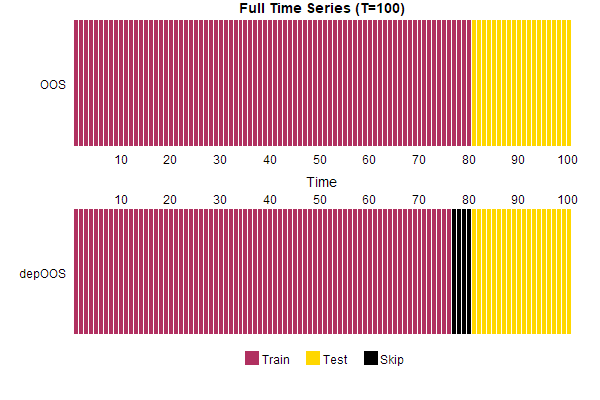
\includegraphics[scale=0.7]{oosplots}
\end{figure}

\subsubsection{SELECTION BASED ON CV FOR INDEPENDENT DATA}

\begin{figure}[htbp!]
	\caption{General $K$-fold Cross-Validation for Model Selection for $K=5$ (top) and $K=10$ (bottom)}
	\label{fig:kcvplots}
	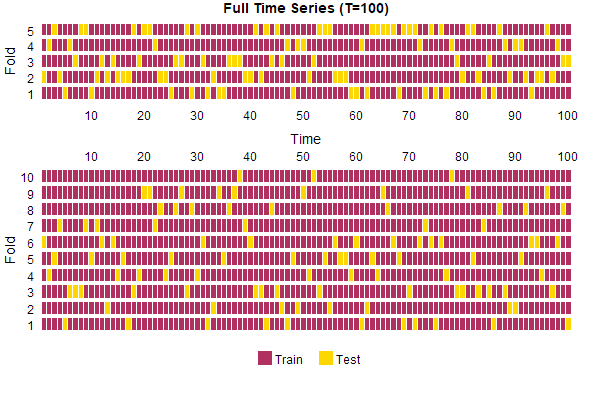
\includegraphics[scale=0.7]{kcvplots}
\end{figure}

\subsubsection{SELECTION BASED ON CV FOR DEPENDENT DATA}

\begin{figure}[htbp!]
	\caption{Non-Dependent $K$-fold Cross-Validation for Model Selection for $K=5$ (top) and $K=10$ (bottom)}
	\label{fig:depkcvplots}
	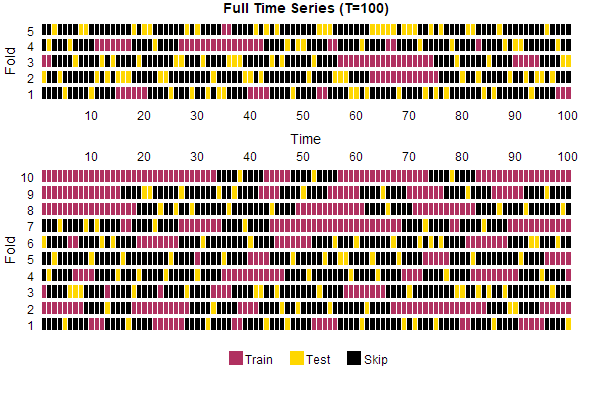
\includegraphics[scale=0.7]{depkcvplots}
\end{figure}

\begin{figure}[htbp!]
	\caption{Non-Dependent $K$-Block Cross-Validation for Model Selection for $K=5$ (top) and $K=10$ (bottom)}
	\label{fig:bcvplots}
	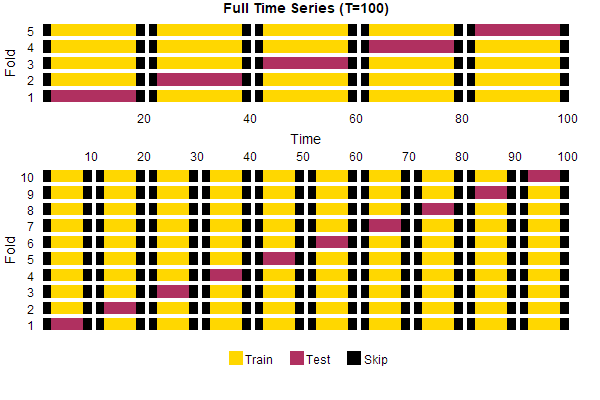
\includegraphics[scale=0.7]{bcvplots}
\end{figure}

\begin{figure}[htbp!]
	\caption{Leave-One-Block-Out Cross-Validation for Model Selection}
	\label{fig:lobocvplots}
	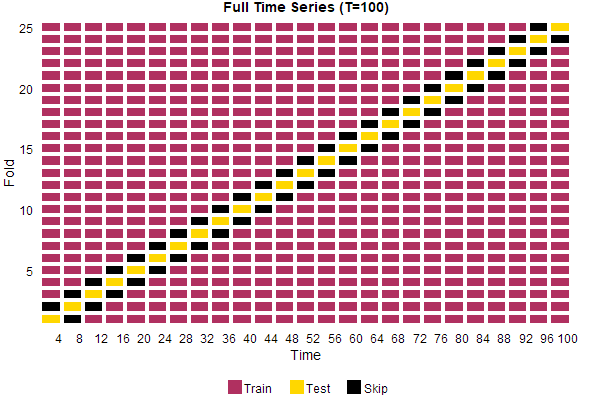
\includegraphics[scale=0.7]{lobocvplots}
\end{figure}

In the time series context, the best model minimizes forecasting error for future observations  unrealized during the model building  

\subsection{BAYESIAN PREDICTIVE POSTERIOR PROJECTION METHOD}
The classic method for model selection within the Bayesian framework begins with a reparameterization of the AR and MA coefficients to $\phi_i^*=\phi_i$ and $\theta_j^*=\theta_j$.

Since the introduction of Bayesian LASSO, research in Bayesian regularization methods has exploded over the last ten years. Bayesian methods analogous to adaptive lasso \citep{Leng2014}, elastic net \citep{Li2010a}, and adaptive elastic net \citep{Stankiewicz2015} have been introduced and applied. \cite{Polson2010}





\section{MONTE CARLO SIMULATIONS}
Multiple Monte Carlo studies are performed to evaluate the effectiveness of the three methods on subset ARMA selection. Consider the three time series $\{y_{1,t}\}$, $\{y_{2,t}\}$, and $\{y_{3,t}\}$ generated by the Gaussian ARMA processes expressed in Equations \ref{eq:simarma1}, \ref{eq:simarma2}, and \ref{eq:simarma3}.
\begin{equation}
	\label{eq:simarma1}
	y_{1,t}=0.8y_{1,t-1}+0.7y_{1,t-6}-0.56y_{1,t-7}+\epsilon_{1,t}
\end{equation}
\begin{equation}
	\begin{split}
	\label{eq:simarma2}
	y_{2,t}&=0.8y_{2,t-1}+0.7y_{2,t-6}-0.56y_{2,t-7}\\
	&+0.8\epsilon_{2,t-1}+0.7\epsilon_{2,t-6}+0.56\epsilon_{2,t-7}+\epsilon_{2,t}
	\end{split}
\end{equation}
\begin{equation}
	\label{eq:simarma3}
	y_{3,t}=0.8\epsilon_{3,t-1}+0.7\epsilon_{3,t-6}+0.56\epsilon_{3,t-7}+\epsilon_{3,t}
\end{equation}
The errors $\{\epsilon_{1,t}\}$, $\{\epsilon_{2,t}\}$, and $\{\epsilon_{3,t}\}$ are i.i.d. Gaussian processes with $0$ mean. These three ARMA models are equivalent to the multiplicative seasonal models of period 6 estimated in \cite{Chen2011} using adaptive Lasso. 









\section{APPLICATION}

Carbon dioxide $\textrm{CO}_2$ levels are constantly measured at strategically placed atmospheric monitoring observatories around the world to track climate change. The {\bf datasets} package in {\bf R} \citep{RCORETEAM} contains a monthly time series of  $\textrm{CO}_2$ levels for January 1959 to December 1997 measured in Mauna Loa, Hawaii, United States. The {\bf TSA} package in {\bf R} \citep{RTSA} contains a similar but shorter series  measured  in Alert, Nunavut, Canada, from January 1994 to December 2004. Let $\{x_{1,t}:t=1,2,\cdots,468\}$ represent the Mauna Loa data, and $\{x_{2,t}:t=1,2,\cdots,132\}$ represent the Alert data. Both $\{x_{1,t}\}$ and $\{x_{2,t}\}$ are nonstationary in mean and cyclical with seasonal periodicity $S=12$. The latter series $\{x_{2,t}\}$ serves as a primary textbook example  to demonstrate the selection, fitting, and forecasting of seasonal models \citep{Cryer2008}. Following the examples provided in \cite{Cryer2008,Chen2011}, subset SARMA$(p,q)\times(P,Q)_{12}$ models utilized at both locations are applied after seasonal and regular differencing . 

Define $y_{k,t}=\nabla_1\nabla_{12}x_{k,t}$ for $k\in\{1,2\}$  where $\nabla_s$ is the difference operator such that $\nabla_s y_t=y_t-y_{t-s}$.  Using all variations of adaptive lasso, adaptive elastic net, and projection model selection, we fit subset ARMA($14,14$) models to $\{y_{1,t}:t=1,2,\cdots,372\}$ corresponding to data prior to 1990 and $\{y_{2,t}:t=1,2,\cdots,108\}$ corresponding to data prior to 2003. The remaining portions $\{y_{1,t}:t=373,374,\cdots,468\}$ and $\{y_{2,t}:t=109,110,\cdots,132\}$ are intentionally preserved for forecasting comparison. Figures \ref{fig:co2plots} and \ref{fig:co2plots2} illustrate the division of the data into fitting and forecasting periods, as well as, the progression of seasonal and regular differencing for Mauna Loa and Alert, respectively.

\begin{figure}[htbp!]
	\centering
	\caption{Plots of $x_{1,t}$ (Top),$\nabla_{12}x_{1,t}$ (Middle), and $\nabla_1\nabla_{12}x_{1,t}$ (Bottom) Partitioned Into Fitting (solid) and Forecasting (dotted) Periods}
	\label{fig:co2plots}
	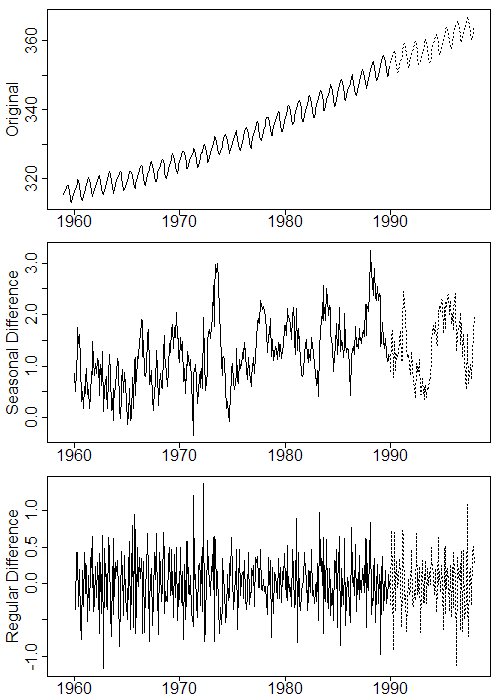
\includegraphics[scale=0.8]{co2plots}
\end{figure}

\begin{figure}[htbp!]
	\centering
	\caption{Plots of $x_{2,t}$ (Top),$\nabla_{12}x_{2,t}$ (Middle), and $\nabla_1\nabla_{12}x_{2,t}$ (Bottom) Partitioned Into Fitting (solid) and Forecasting (dotted) Periods}
	\label{fig:co2plots2}
	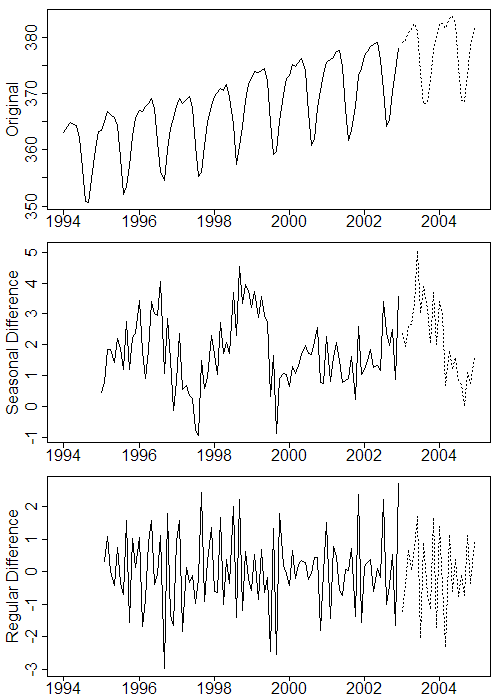
\includegraphics[scale=0.8]{co2plots2}
\end{figure}


The DGPs of $\{y_{1,t}\}$ and $\{y_{2,t}\}$ are hidden to the observer; therefore, evaluating the ability of a subset selection method to uncover the truth is an impossible task. The exploration into various cross-validation methods was motivated by the terminal desire to produce forecasts. Using the final subset ARMA($14,14$) models selected from the full library of methods presented in this paper, we obtain rolling $1$-step ahead predictions $\hat{y}_{k,t}$ over the full forecasting period of length $n_k$ where $k\in\{1,2\}$. As previously determined, $n_1=96$ and $n_2=24$.  Methods are evaluated based on root mean squared error (RMSE), mean absolute percentage error (MAPE), mean bias (MB), and mean directional bias (MDB). The formulas for these metrics are expressed in Equation \ref{eq:fmetrics}. In the expression for MDB, $\textrm{sgn}(x_t)=1$ if $x_t>0$ and $\textrm{sgn}(x_t)=-1$ if $x_t<0$.

\begin{equation}
\label{eq:fmetrics}
\begin{split}
	RMSE_k&=\frac{1}{n_k} \sum\limits_{j=1}^{n_k} (y_k-\hat{y}_k)^2 \\
	MAPE_k&=\frac{100}{n_k} \sum\limits_{j=1}^{n_k} \bigg|\frac{y_{k,j}-\hat{y}_{k,j}}{y_{k,j}}\bigg| \\
	MB_k&=\frac{1}{n_k} \sum\limits_{j=1}^{n_k} (y_{k,j}-\hat{y}_{k,j}) \\
	MDB_k&=\frac{1}{n_k} \sum\limits_{j=1}^{n_k} \textrm{sgn}(y_{k,j}-\hat{y}_{k,j})\\
\end{split}
\end{equation}






\section{CONCLUSION}
